
%% Begin slides template file
\documentclass[11pt,t,usepdftitle=false,aspectratio=169]{beamer}
%% ------------------------------------------------------------------
%% - aspectratio=43: Set paper aspect ratio to 4:3.
%% - aspectratio=169: Set paper aspect ratio to 16:9.
%% ------------------------------------------------------------------

\usetheme[]{uibk}
%% ------------------------------------------------------------------
%% - foot: Add a footer line for conference name and date.
%% - logo: Add the university logo in the footer (only if 'foot' set).
%% - bigfoot/sasquatch: Larger font size in footer.
%% - nototalslidenumber: Hide the total number of slides (only if 'foot' set)
%% - license: Add CC-BY license symbol to title slide (e.g., for conference uploads)
%%   (TODO: At the moment no other licenses are supported.)
%% - licenseall: Add CC-BY license symbol to all subsequent slides slides
%% - url: use \url{} rather than \href{} on the title page
%% - nosectiontitlepage: switches off the behaviour of inserting the
%%   titlepage every time a \section is called. This makes it possible to
%%   use more than one section + thanks page and a ToC off by default.
%%   If the 'nosectiontitlepage' is set you can create UIBK title slides
%%   using the command '\uibktitlepage{}' in your document to create
%%   one or multiple title slides.
%% ------------------------------------------------------------------

%% ------------------------------------------------------------------
%% The official corporate colors of the university are predefined and
%% can be used for e.g., highlighting something. Simply use
%% \color{uibkorange} or \begin{color}{uibkorange} ... \end{color}
%% Defined colors are:
%% - uibkblue, uibkbluel, uibkorange, uibkorangel, uibkgray, uibkgraym, uibkgrayl
%% The frametitle color can be easily adjusted e.g., to black with
%% \setbeamercolor{titlelike}{fg=black}
%% ------------------------------------------------------------------

%\setbeamercolor{verbcolor}{fg=uibkorange}
%% ------------------------------------------------------------------
%% Setting a highlight color for verbatim output such as from
%% the commands \pkg, \email, \file, \dataset 
%% ------------------------------------------------------------------


%% information for the title page ('short title' is the pdf-title that is shown in viewer's titlebar)
\title[Balancing binary values]{Defending against power analysis\\ by balancing binary values}
\subtitle{\large a compiler based approach}

\author[Alexander Schl\"ogl]{\small Alexander Schl\"ogl, supervised by Univ.-Prof. Dr. Rainer B\"ohme}
%('short author' is the pdf-metadata Author)
%% If multiple authors are required and the font size is too large you
%% can overrule the font size of author and url by calling:
%\setbeamerfont{author}{size*={10pt}{10pt},series=\mdseries}
%\setbeamerfont{url}{size*={10pt}{10pt},series=\mdseries}
%\URL{}
%\subtitle{}

\footertext{{\LaTeX} beamer theme}
\date{2019-09-11}

\headerimage{2}
%% ------------------------------------------------------------------
%% The theme offers four different header images based on the
%% corporate design of the university of innsbruck. Currently
%% 1, 2, 3 and 4 is allowed as input to \headerimage{...}. Default
%% or fallback is '1'.
%% ------------------------------------------------------------------

\usepackage{graphicx}
\graphicspath{ {fig/}}

\begin{document}

%% ALTERNATIVE TITLEPAGE
%% The next block is how you add a titlepage with the 'nosectiontitlepage' option, which switches off
%% the default behavior of creating a titlepage every time a \section{} is defined.
%% Then you can use \section{} as it's originally intended, including a table of contents.
% \usebackgroundtemplate{\includegraphics[width=\paperwidth,height=\paperheight]{titlebackground.pdf}}
% \begin{frame}[plain]
%     \titlepage
% \end{frame}
% \addtocounter{framenumber}{-1}
% \usebackgroundtemplate{}

%% Table of Contents, if wanted:
%% this requires the 'nosectiontitlepage' option and setting \section{}'s as you want them to appear here.
%% Subsections and subordinates are suppressed in the .sty at the moment, search
%% for \setbeamertemplate{subsection} and replace the empty {} with whatever you want.
%% Although it's probably too much for a presentation, maybe for a lecture.
%% Please note: \maketitle allows you to render a uibk-style title page wherever needed
%% in the document even if 'nosectiontitlepage' option is set (note: \maketitle will not
%% create a new section and is therefore not included in \tableofcontents (if used).
% \maketitle
% \begin{frame}
%     \vspace*{1cm plus 1fil}
%     \tableofcontents
%     \vspace*{0cm plus 1fil}
% \end{frame}


%% this sets the first PDF bookmark and triggers generation of the title page
\section{Bookmark Title}

%% this just generates PDF bookmarks
\subsection{Overview}

%% first slide
\begin{frame}

  \frametitle{Overview}
  \textbf{Content}
  
  \begin{itemize}
  \item Power analysis
  \item Approach
  \item Arithmetic
  \item Compiler Pass
  \item Results
  \item Future Work
  \end{itemize}

\end{frame}

\subsection{Power Analysis}
\begin{frame}
  \frametitle{Platform}
  
\end{frame}

\begin{frame}
  \frametitle{Power analysis}

\end{frame}

\begin{frame}
  \frametitle{Power analysis cont.}

\end{frame}

\begin{frame}
  \frametitle{Power analysis cont.}
\end{frame}
\begin{frame}
  \frametitle{Power analysis cont.}

\end{frame}

\subsection{Approach}
\begin{frame}
  \frametitle{Approach}
\end{frame}
\begin{frame}
  \frametitle{Approach cont.}

\end{frame}

\subsection{Arithmetic}
\begin{frame}
  \frametitle{Arithmetic}
\end{frame}

\begin{frame}
  \frametitle{Arithmetic cont.}

  \begin{columns}[T] % align columns
    \begin{column}{.05\textwidth}
    \end{column}
    \hfill
    \begin{column}{.38\textwidth}
      Find replacements for:
      \begin{itemize}
      \item \texttt{ORR}
      \item \texttt{AND}
      \item \texttt{XOR}
      \item \texttt{ADD}
      \item \texttt{SUB}
      \item \texttt{MUL}
      \item \texttt{SHIFTS}
      \item \texttt{DIV}
      \item \texttt{REM}
      \end{itemize}
    \end{column}%
    \hfill%
    \begin{column}{.48\textwidth}
      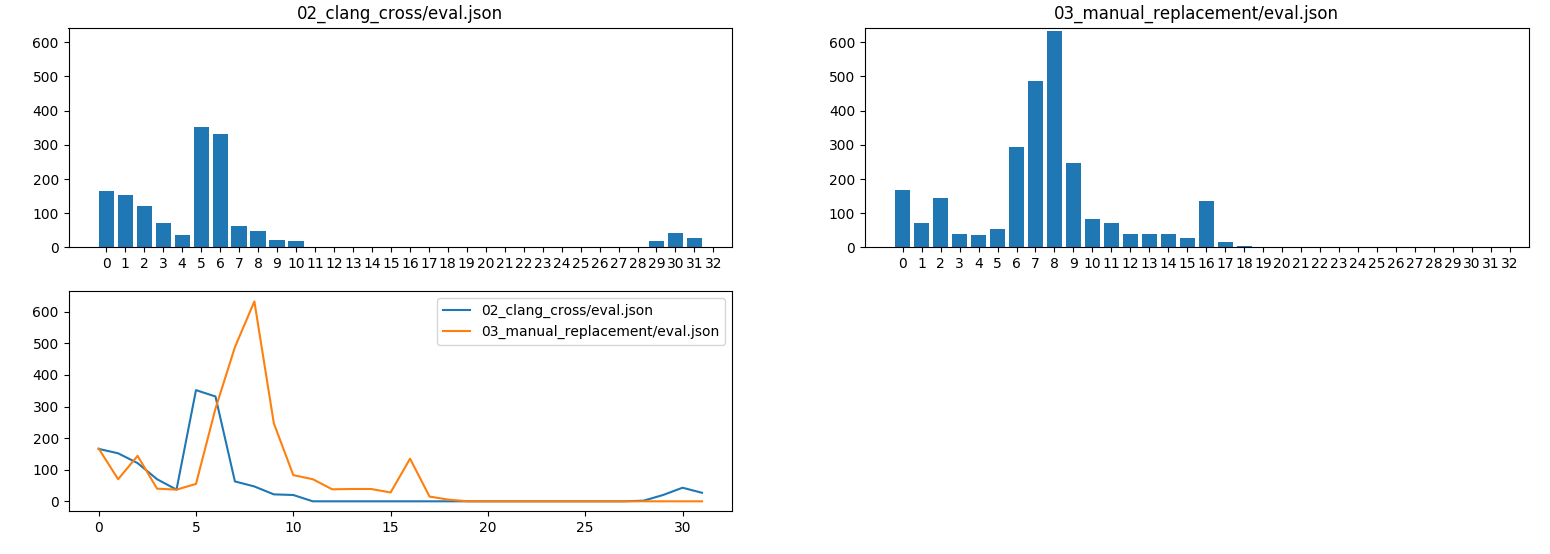
\includegraphics[width=\textwidth, height=0.7\textheight,draft]{placeholder}
    \end{column}%
  \end{columns}
\end{frame}

\begin{frame}
  \frametitle{Verifying the arithmetic}

  
\end{frame}

\subsection{Compiler Pass}
\begin{frame}
  \frametitle{Compiler pass}

\end{frame}
\begin{frame}
  \frametitle{Compiler pass cont.}

  \begin{columns}[T]
    \begin{column}{0.48\textwidth}
      IR code before
      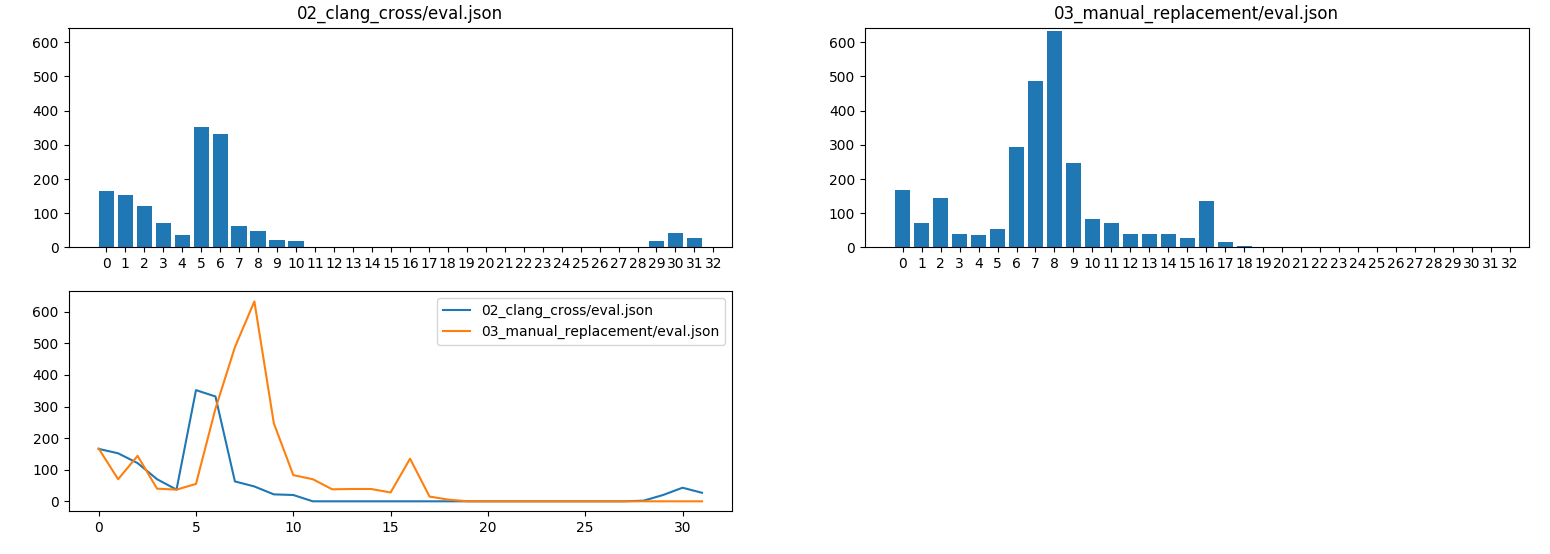
\includegraphics[width=\textwidth, height=\textheight, draft]{placeholder}
    \end{column}
    \hfill
    \begin{column}{0.48\textwidth}
      IR code after
      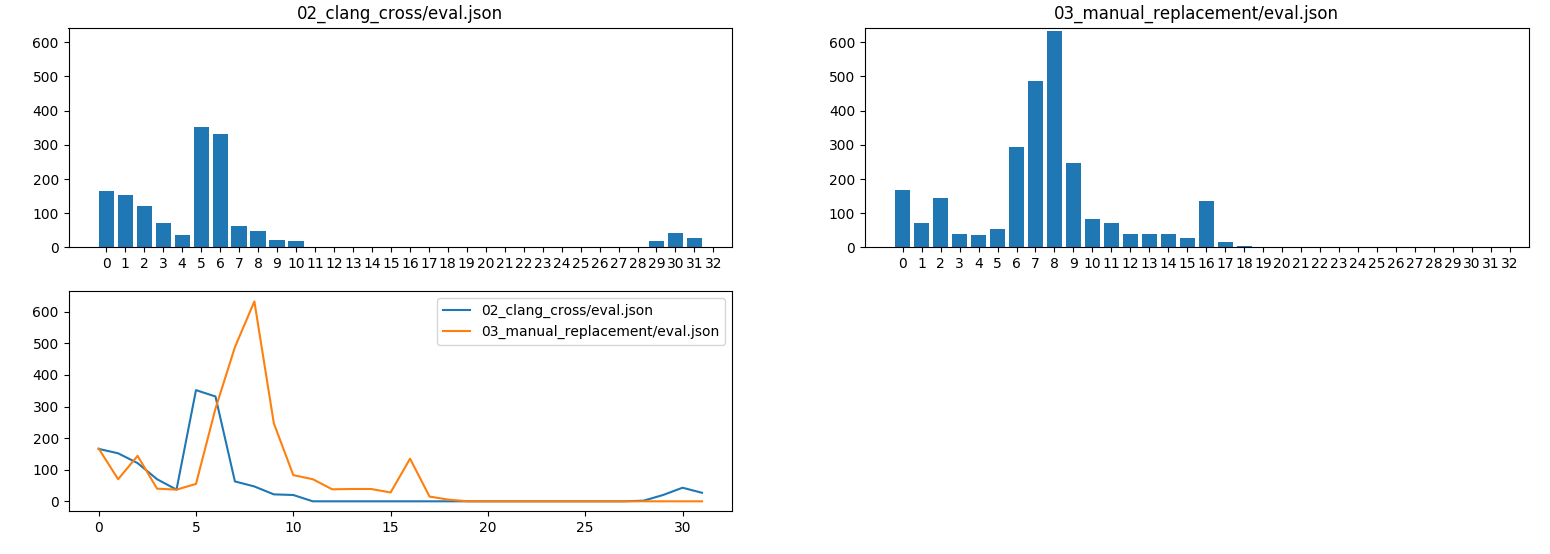
\includegraphics[width=\textwidth, height=\textheight, draft]{placeholder}
    \end{column}
  \end{columns}
\end{frame}
\begin{frame}
  \frametitle{Binary operators}

  \begin{columns}[T]
    \begin{column}{.48\textwidth}
      \begin{itemize}
      \item[] written as C functions
      \item[] linked into same module
      \item[] llvm operators changed to calls
      \end{itemize}
      \vfill
      \begin{block}{Tradeoff}
        \begin{itemize}
        \item[+] simplicity
        \item[+] modularity
        \item[+] small binaries
        \item[-] (currently) on inlining
        \item[-] overhead
        \end{itemize}
      \end{block}
    \end{column}
    \hfill
    \begin{column}{.48\textwidth}
      rtlib.c
      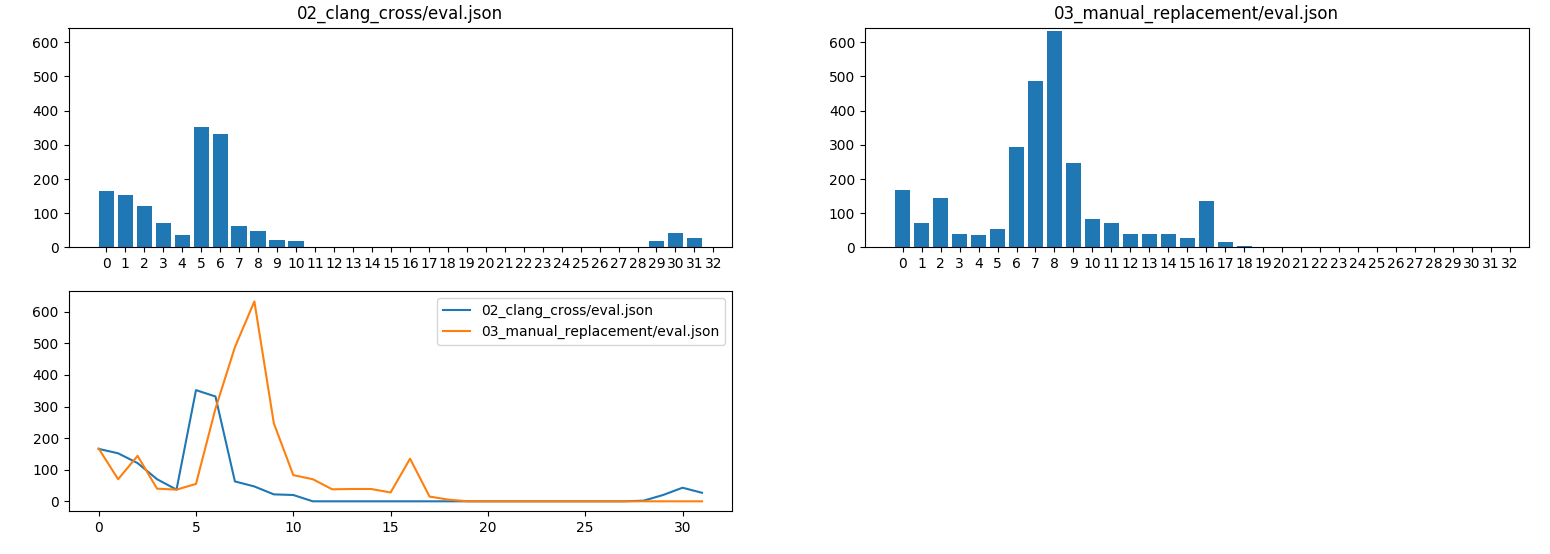
\includegraphics[width=\textwidth,draft]{placeholder.png}
      llvm-link
      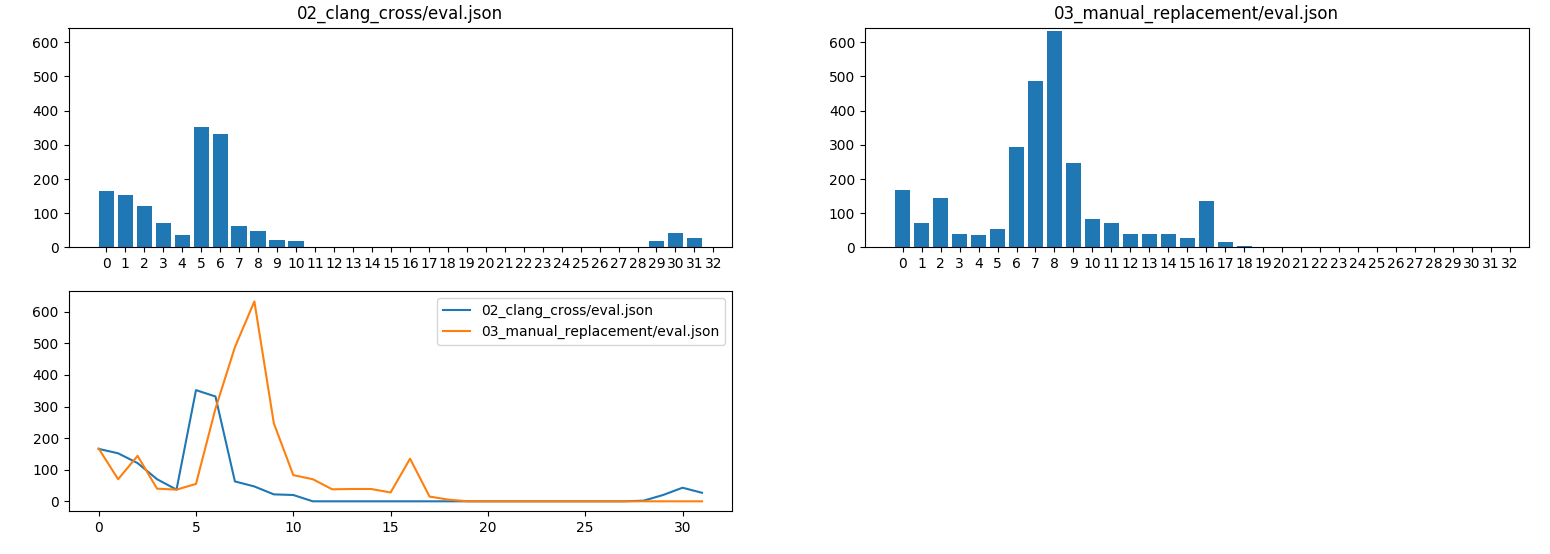
\includegraphics[width=\textwidth,draft]{placeholder.png}
      Balance.cpp
      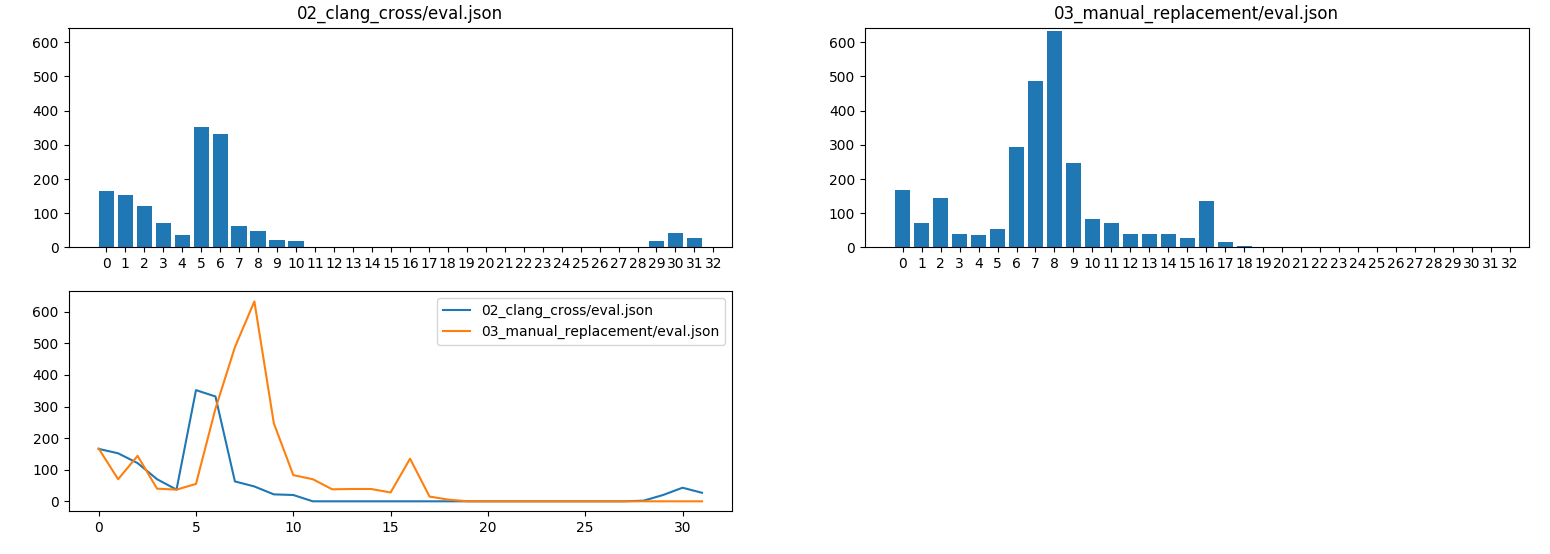
\includegraphics[width=\textwidth,draft]{placeholder.png}
    \end{column}
  \end{columns}
\end{frame}

\subsection{Evaluation}
\begin{frame}
  \frametitle{Evaluation}

  How to generate ``virtual'' power traces?
  
  \begin{alertblock}{Qemu alone}
    \begin{itemize}
    \item[+] fast
    \item[-] wrong resolution
    \end{itemize}
  \end{alertblock}

  \begin{block}{Qemu + gdb}
    \begin{itemize}
    \item[+] correct resolution
    \item[+] includes program location information
    \item[-] \textbf{very} slow
    \end{itemize}
    Execute instruction by instruction, dump registers every time
  \end{block}
\end{frame}

\begin{frame}
  \frametitle{Results}
  \center
  \vfill
  \begin{tabular}{|l|l|l|}
    \hline
    & \multicolumn{2}{c|}{AES} \\
    \cline{2-3}
    & unbalanced & balanced \\
    \cline{2-3}
    No. of instructions & 22 876 & 339 168 \\
    Relative increase & 1 & 14.888 \\
    Balanced operations & 20 571 & 334 521 \\
    Unbalanced operations & 2211 & 4647 \\
    Balancedness      & 0.903 & 0.986 \\
    Code size         & 76 KB & 78 KB \\
    \hline
  \end{tabular}
  \vfill
\end{frame}

\subsection{Results}
\begin{frame}
  \frametitle{Results cont.}

\end{frame}

\begin{frame}
  \frametitle{Results cont.}
  \frametitle{}

\end{frame}
\begin{frame}
  \frametitle{Results cont.}
  \frametitle{}

\end{frame}
\begin{frame}
  \frametitle{Results cont.}

\end{frame}
\begin{frame}
  \frametitle{Results cont.}

\end{frame}
\begin{frame}
  \frametitle{Results cont.}

\end{frame}

\subsection{Future Work}
\begin{frame}
  \frametitle{Future work}
  Same idea with different methods:
  \begin{itemize}
  \item Test on actual hardware
  \item Balance globals
  \item Mark balancing targets
  \item Move balancing to type system
  \end{itemize}
  \vspace{0.5cm}
  Different ideas with same method:
  \begin{itemize}
  \item Other power analysis defenses
  \item Control flow randomization
  \item Move more security tools to LLVM
  \end{itemize}
\end{frame}

\subsection{Conclusion}
\begin{frame}
  \frametitle{Conclusion}

\end{frame}

\end{document}
